% -*- latex -*-
%%%%%%%%%%%%%%%%%%%%%%%%%%%%%%%%%%%%%%%%%%%%%%%%%%%%%%%%%%%%%%%%
%%%%%%%%%%%%%%%%%%%%%%%%%%%%%%%%%%%%%%%%%%%%%%%%%%%%%%%%%%%%%%%%
%%%%
%%%% This text file is part of a package of parallel performance studies
%%%%
%%%% by Victor Eijkhout, copyright 2018-2020
%%%%
%%%% report-body.tex : main text of report on MPI performance of non-contiguous sends
%%%%
%%%%%%%%%%%%%%%%%%%%%%%%%%%%%%%%%%%%%%%%%%%%%%%%%%%%%%%%%%%%%%%%
%%%%%%%%%%%%%%%%%%%%%%%%%%%%%%%%%%%%%%%%%%%%%%%%%%%%%%%%%%%%%%%%

\section{Introduction}

Most \ac{MPI} benchmarks use the send of a contiguous buffer to measure
how close the MPI software gets to the theoretical speed of the
hardware.
However, in practice we often need to send non-contiguous data, such
as the real parts of a complex array, every other element of a grid
during multigrid coarsening, or irregularly spaced elements in a
\ac{FEM} boundary transfer.

To support this, MPI has so-called `derived datatypes' routines, that
describe non-contiguous data. While they offer an elegant interface,
programmers always worry about any performance implications of using
these derived types. In this report we perform an experimental
investigation of  various schemes for sending non-contiguous
data, comparing their performances both to each other, as well as to
the performance of a contiguous send, which we will consider as the
optimal, reference, rate.

\subsection{Performance determining factors}

We introduce the term `performance quotient', by which we mean
the ratio of the time for a non-contiguous scheme and for a
contiguous send of the same effective size. The value of this quotient
is a combination of bandwidth issues, buffer handling, and type handling.

Specifically, we investigate the following non-orthogonal issues:
\begin{enumerate}
\item Manually copying irregular data to a contiguous buffer and
  sending the latter, versus using MPI derived datatypes to send irregular data;
\item using both two-sided and one-sided point-to-point; and
\item using ordinary, buffered, and packed sends to counteract adverse effects of
  MPI's internal buffering.
\end{enumerate}

\subsection{Outline}

We discuss our schemes in section~\ref{sec:schemes} and our
experimental setup in section~\ref{sec:setup}. Results are graphed and
discussed in section~\ref{sec:results}. We give our overall conclusion
in section~\ref{sec:conclusion}.

\section{Send schemes}
\label{sec:schemes}

We describe the various send schemes that we are available. 

\subsection{Contiguous send}

To establish a baseline we send a contiguous buffer, and accept the
result as the attainable performance of the hardware/software
combination.

The cost of this scheme is
\begin{enumerate}
\item loading $N$ elements from memory to the processor, and
\item sending $N$ elements through the network.
\end{enumerate}
The two are probably overlapped, and to first order of approximation
we equate memory bandwidth and network transmission speed, so we
assign a proportionality constant of~1 to this scheme.

\subsection{Pipelined sends from non-contiguous addresses}

Sending non-contiguous data,
we note that
only $N$ elements are directly access for reading, but
since cachelines are 8~elements long, in effect all $2N$ elements
of the input array are transferred from memory.

With enough support of the \ac{NIC} and its firmware, it
would be possible to pipeline the $2N$ reads and $N$ sends
similarly to the reference case. This scheme would have a proportionality constant of~2.

That this is possible in principle was shown in~\cite{LI:MpiDataUMR}.
In practice we don't see this performance,
and our observed performance numbers are
completely in accordance with an assumption of non-pipelining.

\subsection{Manual copying}

Since we are sending non-contiguous data, the minimal solution is to
copy the data between a user array and the send buffer. We allocate
the send buffer outside the timing loop, and reuse it.

The cost for this is
\begin{enumerate}
\item the cost of the copying loop, and
\item the cost of the contiguous send.
\end{enumerate}
The copying loop loads $2N$ elements from memory and writes~$N$.
The
latter writes can be interleaved with the loads, so most likely only
the loads contribute to the measured time.
%
Next, the building of the send buffer has to be fully finished before
the \n{MPI_Send} can be issued, so with the assumptions made before,
we expect a slowdown of a factor of~3 over the reference speed.

In this case, our performance quotient is completely determined by
bandwidth; there is no additional buffer handling inside the MPI
implementation, and the type handling is minimal too.

A further point to note is that the copying loop is of necessity in
user space, so any offload of sends to the \ac{NIC} is of limited
value, with a possible reduction of the proportionality constant
to~2. We never observed this low value in our tests.

\subsection{Derived datatypes}

MPI has routines such as \n{MPI_Type_create_vector} and
\n{MPI_Type_create_subarray} to offer a convenient interface to
non-contiguous data. As observed above, such derived types could
be streamed but this does not happen in practice.

The best we can hope for is that these routines copy
data to an internal MPI buffer, which is subsequently sent.
This would lead us to  expect a performance similar to the manual copying scheme.

However, the MPI library is `state-less' implying that the large
buffer that is needed for sending can not be maintained between one
send call and another. Thus we expect further performance degradation
from the repeated re-allocation of the internal send buffers,
beyond the basic factor of~3 degradation.
Since many MPI implementations are closed source, and the behaviour
depends on the precise scheme, we can not further analyze this
internal buffer allocation.
(In fact, even for
the open MPICH implementation we found the buffer management code too
inscrutable for analysis.)

\subsection{Buffered sends}

One way obviate problems with internal MPI buffer allocation
is to put this buffer in user space. This is what is done
by MPI `buffered' send routines.
Here a user buffer is one-time attached with
\n{MPI_Buffer_attach} and the send is replaced by \n{MPI_Bsend}.
This buffer needs to be large enough to accomodate all simultaneously
occurring communication.

\subsection{Persistent sends}

MPI uses the mechanism of `persistent' sends to declare a communication
pattern once with \n{MPI_Send/Recv_init},
and then repeatedly initiate it with \n{MPI_Start/Start_all},
which contains no further declaration of source/target or
send/receive buffer specifications.

Ideally, with this knowledge MPI could create a large enough
internal buffer at the \n{MPI_Send/Recv_init} call.
This buffer could be freed when the request associated
with the persistent communication is free,
but in practice this does not seem to happen.

\subsection{One-sided transfer}

We explored using one-sided point-to-point calls. There are two options:
\begin{enumerate}
\item Transfering the data elements in a loop. However, this requires
  a function call per elements so we did not pursue this.
\item Transfering a single derived type.
\end{enumerate}

While one-sided messages have the potential to be more efficient,
since they dispense with a rendez-vous protocol, they still require
some sort of synchronization. We use \n{MPI_Win_fence}.

This protocol is likely susceptible to all the problems
of internal buffer allocation.

\subsection{Packing}

Finally, we considered the use of the \n{MPI_PACKED} data type, used
two different ways.
\begin{itemize}
\item We use a separate \n{MPI_Pack} call for each element. Since this
  uses a function call for each element sent, this scheme has much
  lower performance, observed to be
  at least $4\times$ worse than other schemes.
  For this reason  we did not include it in our plots.
\item We use a single \n{MPI_Pack} call on a derived (vector) datatype.
\end{itemize}

The \n{MPI_Pack} command packs data in an explicitly allocated
send buffer in userspace. This means that we no longer rely on MPI for
buffer management. If the implementation of the pack command is
sufficiently efficient, we expect this scheme to track the manual
copying scheme.

\section{Experimental setup}
\label{sec:setup}

\subsection{Hardware}

We use the following clusters at TACC:
\begin{itemize}
\item Lonestar5: a Cray XC40 with Intel compilers and Cray mpich7.3.
\item Stampede2-knl: a Dell cluster with Knightslanding nodes
  connected with Omnipath, using Intel compilers and Intel MPI.
\item Stampede2-skx: a Dell cluster with dual Skylake nodes connected
  with Omnipath, using Intel compilers and both Intel MPI and mvapich.
\begin{p9}
  \item Power9: a small cluster with IBM SpectrumMPI and Infiniband EDR.
\end{p9}
\end{itemize}

\subsection{Performance measurement}

We measured the time for 20 ping-pongs, where:
\begin{itemize}
\item The `ping' was the
  non-contiguous send. This used an ordinary \n{MPI_Send} for all
  two-sided versions except \n{MPI_Bsend} for the buffered protocol,
  and \n{MPI_Put} for the one-sided version.
\item In all two-sided schemes the target process executed an \n{MPI_Recv} on a contiguous
  buffer.
\item In the two-sided schemes, there was a zero byte `pong' return
  message. In the one-sided scheme we surrounded the transfer with
  active target synchronization fences; the timers surrounded these fences.
\end{itemize}

Time reported in the figures below is the
total time divided by the number of ping-pongs.

\begin{details}
  Every ping-pong was timed individually. We used \n{MPI_Wtime}, which
  on our platforms had a resolution of $1\cdot10^{-6}$ seconds, and the
  minimum measurement ever (for the very smallest message) was around
  $6\cdot10^{-6}$ seconds.
  %
  Our code is set up to dismiss measurements that are more
  than one standard deviation from the average.
\end{details}

\subsection{Buffer and memory management}

All buffers were allocated outside the timing loop,
which is a reasonable assumption in practical applications, where the
same transfer will likely happen multiple times.

Buffers are  64 byte aligned. Page instantiation was kept outside the
timing loop by setting all arrays explicitly to zero.
In between every two ping-pongs an array of size 50M is
rewritten. This is enough to flush the caches on our systems.

\section{Results and discussion}
\label{sec:results}

\def\scaling{.55}
\begin{figure*}[tb]
  \hbox\bgroup
  \kern-10pt
  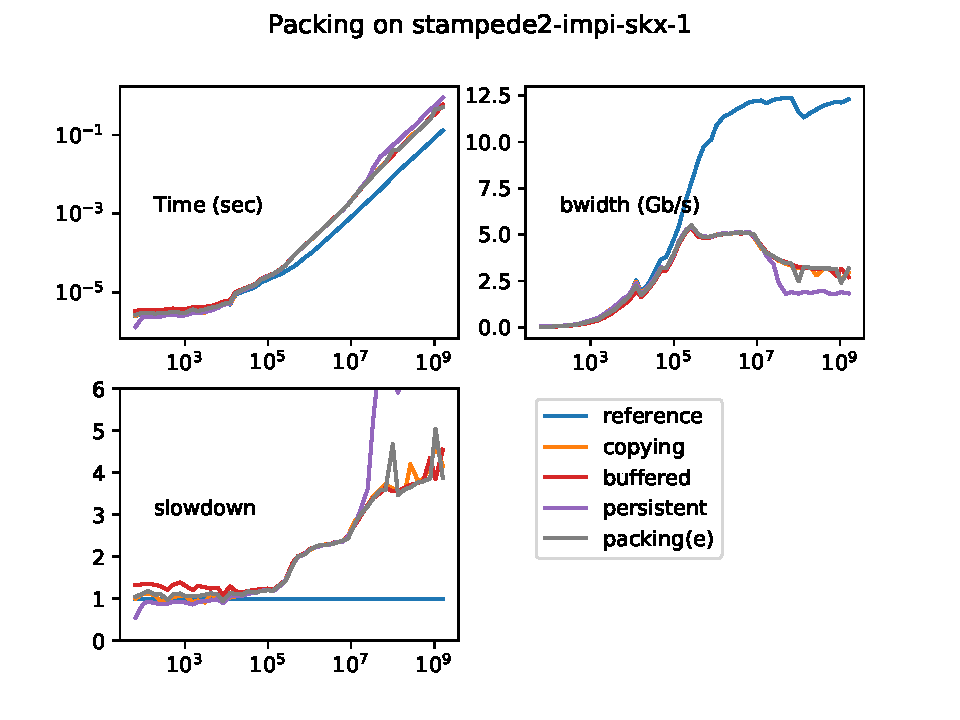
\includegraphics[scale=\scaling]{stampede2-impi-skx-1}
  \kern-20pt
  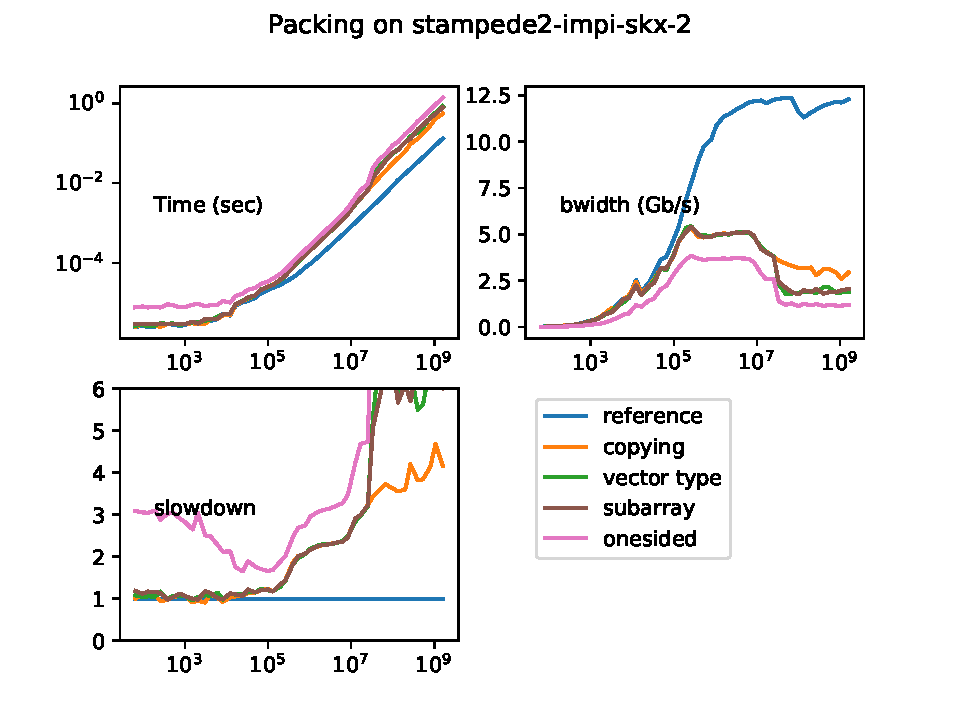
\includegraphics[scale=\scaling]{stampede2-impi-skx-2}
  \egroup
  \caption{Time and bandwidth on Stampede2-skx using Intel MPI}
  \label{fig:skx}
\end{figure*}

\begin{figure*}[tb]
  \hbox\bgroup
  \kern-10pt
  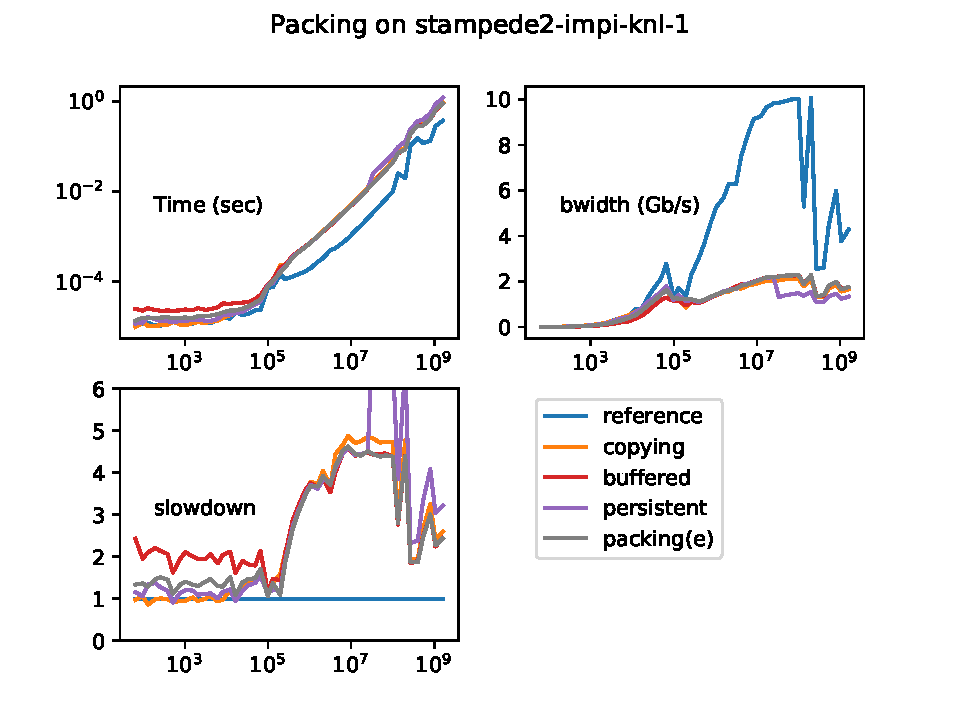
\includegraphics[scale=\scaling]{stampede2-impi-knl-1}
  \kern-20pt
  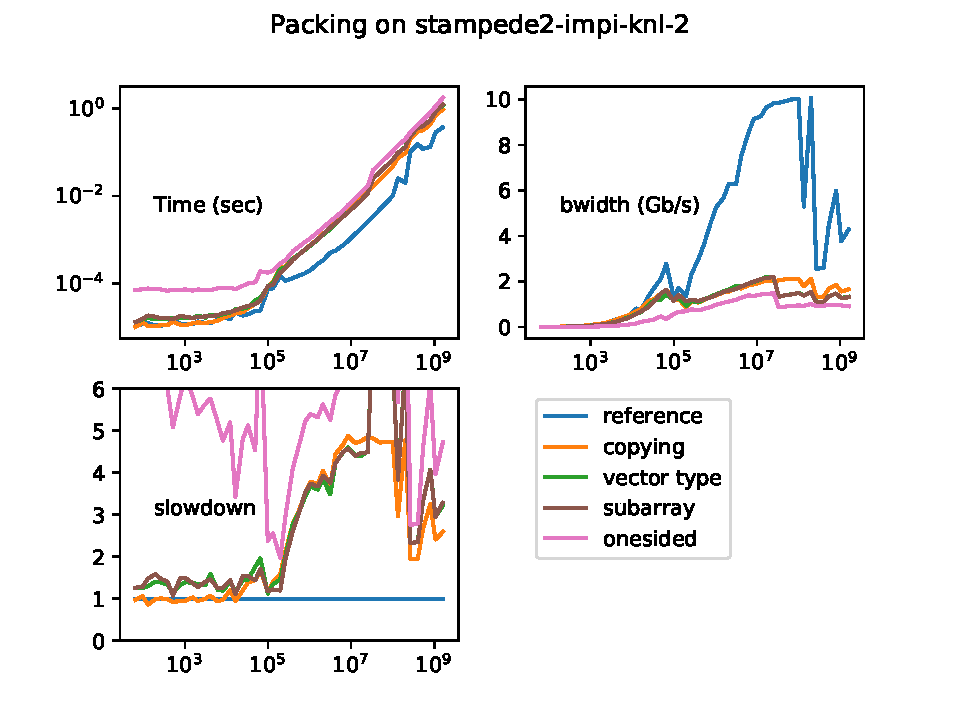
\includegraphics[scale=\scaling]{stampede2-impi-knl-2}
  \egroup
  \caption{Time and bandwidth on Stampede2-knl using Intel MPI}
  \label{fig:knl}
\end{figure*}

\begin{figure*}[tb]
  \hbox\bgroup
  \kern-10pt
  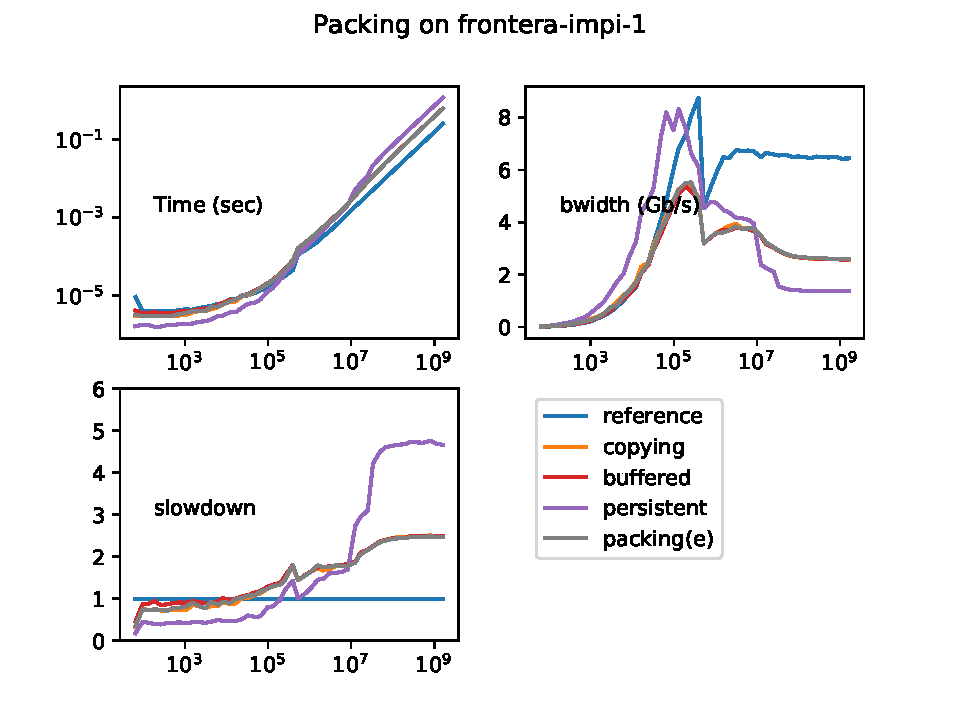
\includegraphics[scale=\scaling]{frontera-impi-1}
  \kern-20pt
  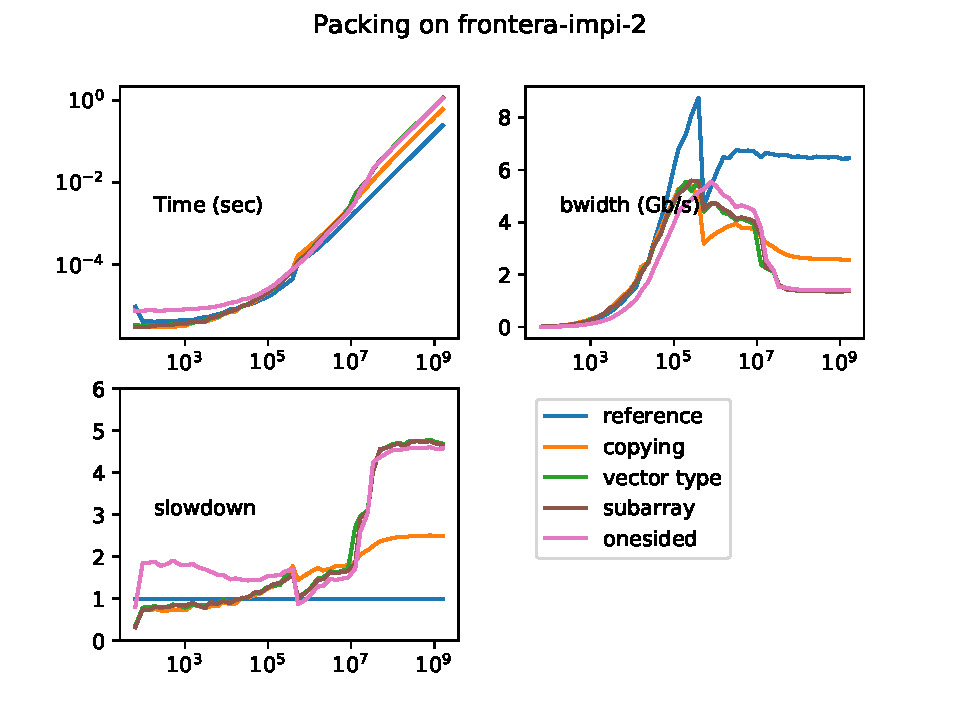
\includegraphics[scale=\scaling]{frontera-impi-2}
  \egroup
  \caption{Time and bandwidth on Frontera using Intel MPI}
  \label{fig:clx-i}
\end{figure*}

\begin{figure*}[tb]
  \hbox\bgroup
  \kern-10pt
  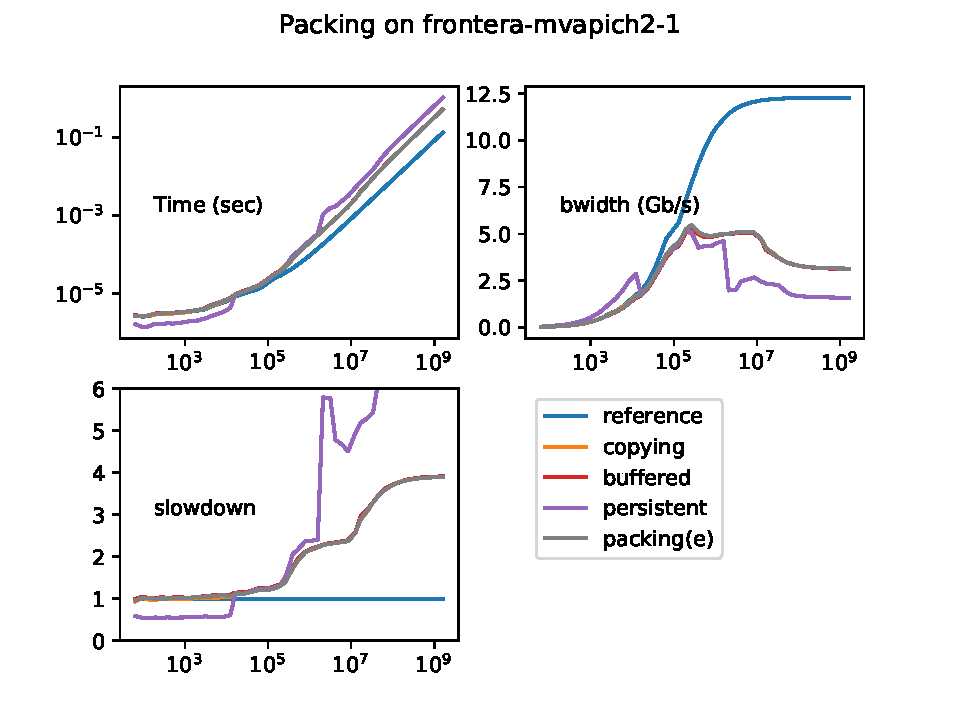
\includegraphics[scale=\scaling]{frontera-mvapich2-1}
  \kern-20pt
  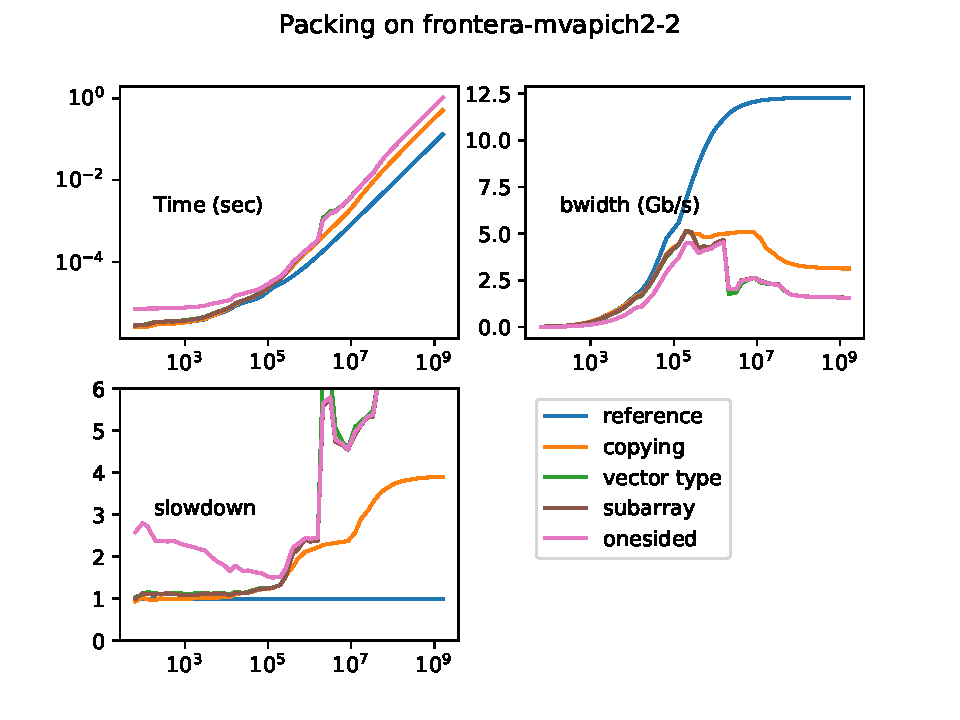
\includegraphics[scale=\scaling]{frontera-mvapich2-2}
  \egroup
  \caption{Time and bandwidth on Frontera using mvapich2}
  \label{fig:clx-v}
\end{figure*}

\begin{figure*}[tb]
  \hbox\bgroup
  \kern-10pt
  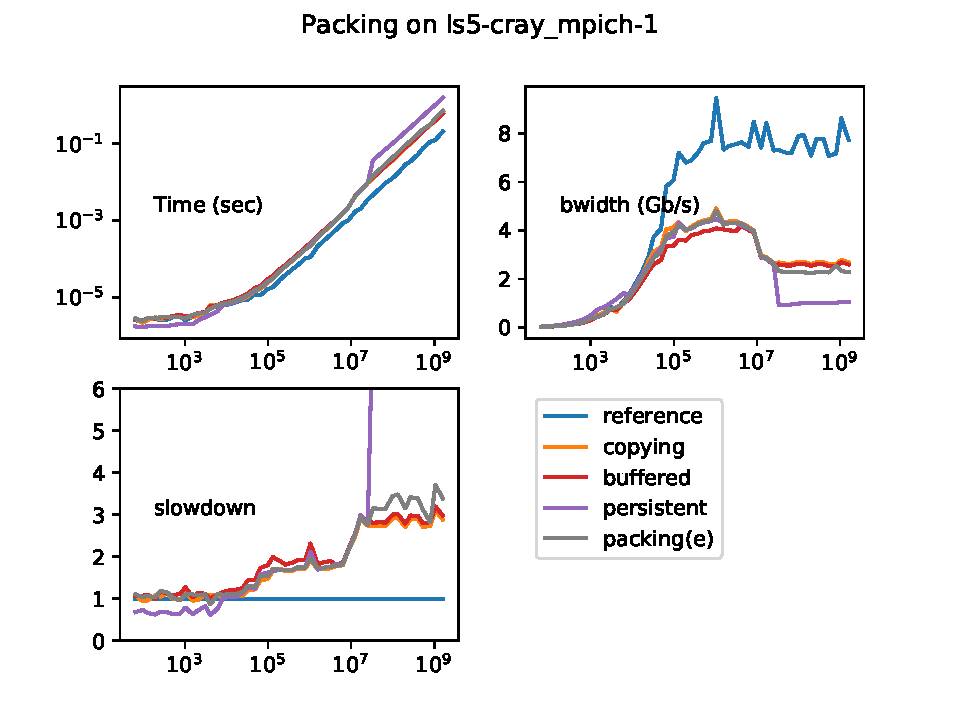
\includegraphics[scale=\scaling]{ls5-cray_mpich-1}
  \kern-20pt
  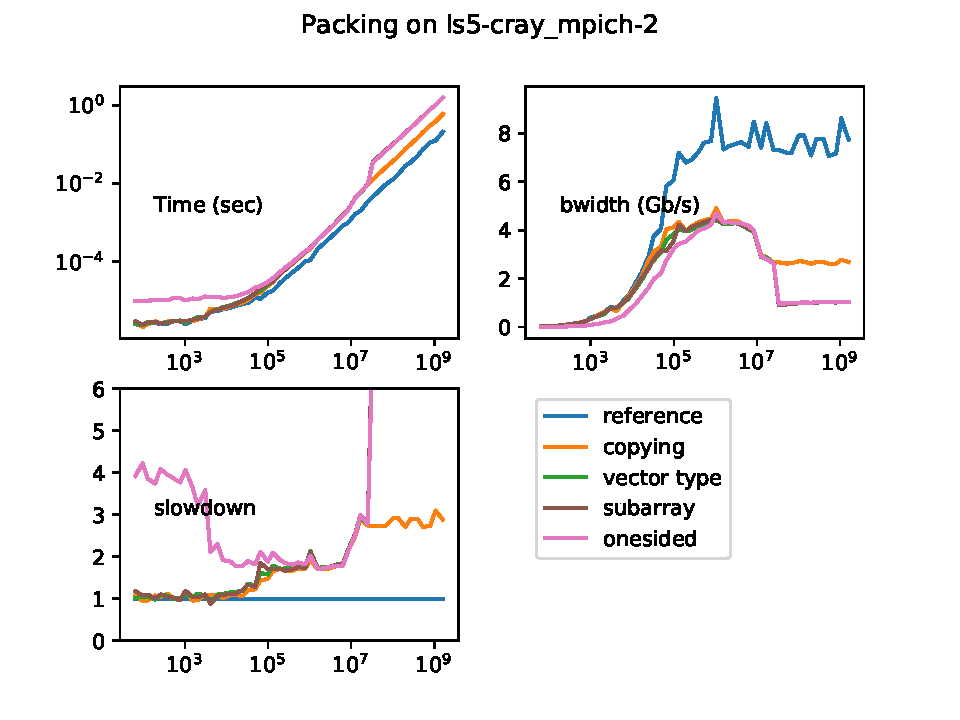
\includegraphics[scale=\scaling]{ls5-cray_mpich-2}
  \egroup
  \caption{Time and bandwidth on a Cray XC40 using the native MPI}
  \label{fig:ls5}
\end{figure*}

\begin{p9}
  \begin{figure*}[tb]
    \hbox\bgroup
    \kern-10pt
    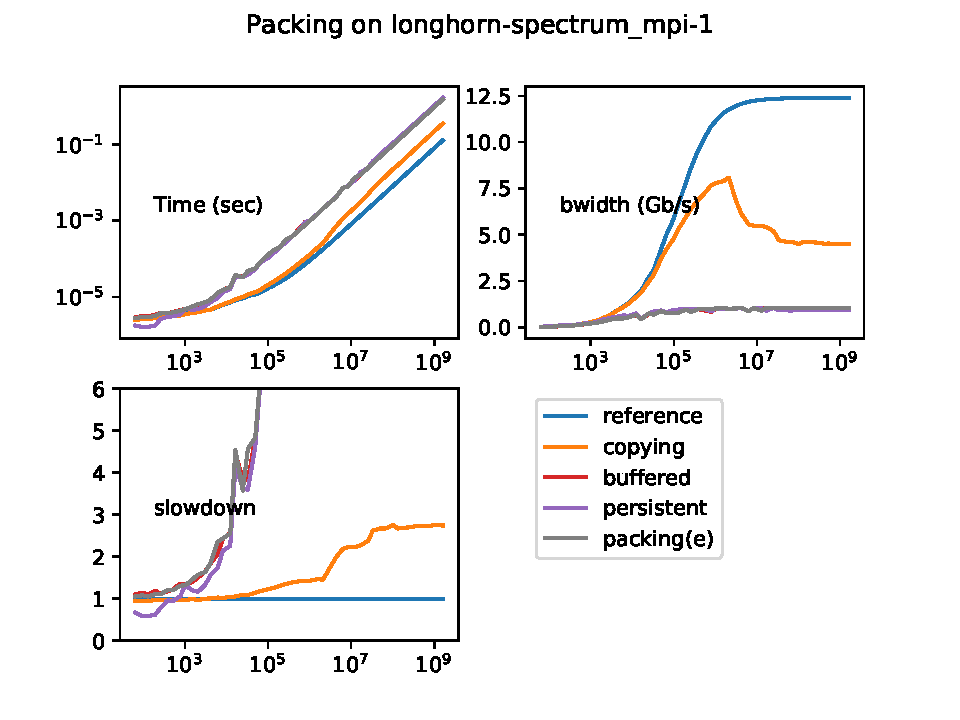
\includegraphics[scale=\scaling]{longhorn-spectrum_mpi-1}
    \kern-20pt
    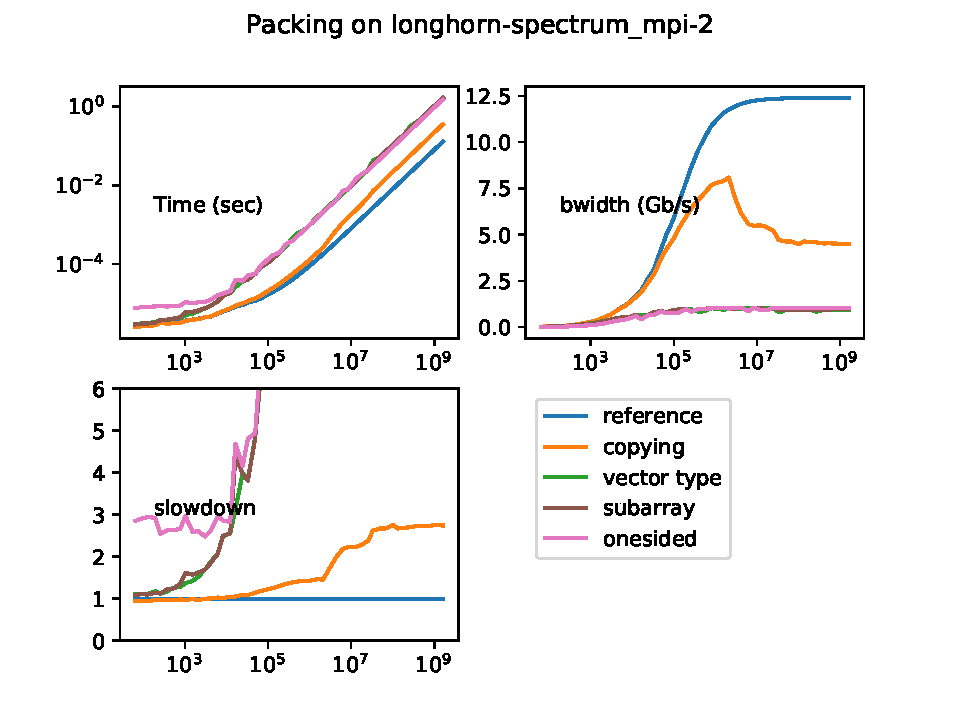
\includegraphics[scale=\scaling]{longhorn-spectrum_mpi-2}
    \egroup
    \caption{Time and bandwidth on an IBM Power9 using Spectrum MPI}
    \label{fig:p9}
  \end{figure*}
\end{p9}

We report benchmark performance on the following clusters,
all located at the Texas Advanced Computing Center:
\begin{itemize}
\item Frontera: an Intel Cascade Lake cluster with Infiniband HDR.
  We use both Intel MPI 18.0.5 (figure~\ref{fig:clx-i})
  and mvapich2.X (figure~\ref{fig:clx-v}). Intel 19 was available
  but exhibited various bugs, for instance in the one-sided protocol.
\item Stampede-skx: an Intel Skylake cluster with Omnipath, using Intel MPI 18.0.5.
\item Stampede-knl: an Intel Knights Landing cluster with Omnipath,
  using Intel MPI 18.0.5.
\item Lonestar: a Cray XC40 cluster with Intel Haswell processors and Cray mpich
  over their proprietary network.
\begin{p9}
\item Longhorn: a Power9 cluster with Spectrum MPI.    
\end{p9}
\end{itemize}

The graphs show for each installation:
\begin{itemize}
\item The measured time of one ping-pong, as function of message size
  in bytes;
\item the effective bandwidth; and
\item the slowdown with respect to the contiguous send. The value of
  this plot is mostly for smaller messages, where differences between
  schemes are not apparent in the first two plots. Note that
  occasional
  blips in the reference curve are reflected in the slowdown numbers.
\end{itemize}
Since several schemes have almost identical performance, we
give the above three graphs twice for each setup:
\begin{itemize}
\item In both cases we give the reference, and the \emph{de factor} reference
  of the copying scheme; then
\item In the left set we give the schemes that have, or are likely to have,
  buffering in user space. This is the buffering, persistent, and packing scheme;
\item In the right set we then plot the derived datatypes (vector and subarray),
  and the one-sided scheme.
\end{itemize}

\subsection{Buffering strategies}

We argue that performance differences can often be attributed to buffering strategies:
the manual copying scheme allocates the buffer once and uses
it repeatedly, whereas MPI, being stateless, need to allocate its buffers for each send.
The overhead of the type mechanisms is of less importance.

We can offer experimental proof of this 
by moving the \n{malloc} and \n{free} inside the
loop over multiple experiments: in this case the copying
method drops in performance to become similar to the derived type
schemes.

\subsection{Method comparisons}

Starting with our observation of the importance of buffering strategies
we expect in the left panels the copying, \textbf{persistent}, \textbf{buffered},
and \textbf{packing} strategies
to perform similarly. The surprise here is that the persistent sends perform worse for large messages,
often with a marked drop at a certain message size.

In the right panels we expect the datatype-based schemes to perform worse than
manual copying, and indeed they do. Using a \textbf{vector} and a \textbf{subarray} datatype
makes no difference, indicating that the subarray type incurs no cost for its
greater generality.

The outlier in the right panels is the \textbf{one-sided} communication.
The various overheads in this scheme give it as expected
a lower performance on small messages, modestly in most cases, and
dramatically so on the KNL processor which has a lower scalar computing
efficiency than all other processors.
On most machines, the one-sided communication was also less efficient
for large messages, though we can not see an intuitive explanation for this.
The exception here is Frontera, where perhaps the new ucx lower layer
makes the synchronization more efficient.

\subsection{Different regimes}

For small message, under about $10^5$ bytes, most schemes perform
similarly. This shows that datatype handling has no major overhead.
\begin{itemize}
\item The one-sided scheme is typically slower than the others on small messages,
  probably because
  of the more complicated synchronization mechanism of
  \n{MPI_Win_fence}, which imposes a large overhead,
  even on only two processes.
\item The persistent scheme is sometimes faster than the reference performance,
  since it does away with some of the rendezvous overhead.
\end{itemize}

For intermediate size message, $10^5\cdots 10^7$ bytes,
all schemes start to show a lower performance than the reference,
by roughly the factor~3 that we predicted above.
They still track each other fairly well. 

For large messages, over $10^7$ bytes,
the reference performance starts to show irregularities
for unclear reasons. This is particularly pronounced on Stampede2-KNL.
The strided schemes also show a drop from their peak performance
that was attained around $10^6$ bytes.

\begin{comment}
  \subsection{Eager limit}

  Most MPI implementations have a switch-over between the `eager
  protocol', where messages are send without handshake, and a
  `rendezvous' protocol that does involve acknowledgement.
  From its nature, the eager protocol relies on sufficient buffer space,
  so there is an `eager limit'. One typically observes that messages
  just over the eager limit can perform worse (at least per byte) than
  once just under.

  The effects of the eager limit are visible in most plots, with the
  following remarks:
  \begin{itemize}
  \item As is to be expected, we mostly see a performance drop at the
    eager limit for all send schemes. For one-sided puts it is less
    pronounced, and for the packing scheme it largely drowns in the
    overhead.
  \item On Cray-mpich we see the performance drop for the reference
    speed, and at double the data sizes for the packing scheme. For the
    other schemes not much of a drop is visible. The reason for this is
    unclear.
  \end{itemize}

  We have tested setting the eager limit over the maximum message size,
  but this did not appreciably change the results for large messages.
\end{comment}

\subsection{Cache flushing}

%% \begin{figure}[p]
%%     \includegraphics[scale=\scaling][scale=.8]{skx-i3}
%%     \includegraphics[scale=\scaling][scale=.8]{skx-i}
%%   \caption{Performance results with (top) and without (bottom) cache
%%     flushing.}
%%   \label{fig:flush}
%% \end{figure}

In tests not reported here we dispensed with flushing the cache in
between sends. This had a clear positive effect on intermediate size messages,
but is unrealistic in practical applications.

\subsection{Ease of use}

The starting point for this study was the question whether
the ease of use of derived datatypes carried a performance penalty.
From the tests reported here we conclude that derived datatypes
can indeed perform close to the optimum of manually copying,
but need to be combined with either message packing,
or buffered sends.

\subsection{Further tests}

This paper is of course not a full exploration of all possible
scenarios in which derived datatypes can be used. In fact, it only
examines the very simplest case of a derived type.
\begin{enumerate}
\item Types with less regular spacing may give worse performance due
  to decreased use of prefetch streams in reading data.
\item Types with larger block sizes may perform better due to higher
  cache line utilization in the read.
\end{enumerate}
A more interesting objection to these tests is that we used exactly
one communicating process per node. This is a realistic model for
certain hybrid cases, but not for `pure MPI' codes. However, a limited
test, not reported in graph form here, shows that no performance
degradation results from having all processes on a node
communicate. (In fact, sometimes a slightly higher bandwidth results.)

The interested reader can find the code in an open repository and
adapt it to their own purposes~\cite{packingrepo}.

\section{Conclusion}
\label{sec:conclusion}

Schemes for sending non-contiguous data between two processes are
considerably slower than sending contiguous data. The slowdown of at
least a factor of three can mostly be explained by multiple memory
reads and a lack of overlap of memory and network traffic.
Attaining such overlap for non-contiguous data depends on advanced
functionality of the network interface~\cite{Hashmi:mpitype-ipdps19,LI:MpiDataUMR}.

For small to intermediate size messages, the various schemes
perform fairly similarly, so there should be no reason not to use
derived datatypes, these being the most user-friendly.
For small messages the decreased overhead of persistent communication
may help.

For larger messages the buffer management of MPI becomes a concern,
so, failing hardware support,
the derived types should be used either in buffered sends
or through the packing scheme.
